\newpage
\section{Question 3}
\lstinputlisting{./MATLABFiles/q2.m}
	\pagebreak
	\subsection*{DH Notation}
	\noindent
		\begin{table}[position = here]
		\begin{centering}
		\begin{tabular}{||l|l|l|l|l||}
			\hline \rule[-2ex]{0pt}{5.5ex} \color{red}\bf{i} & \color{red}\bf{$\theta$}		&	\color{red}\bf{d}	&	\color{red}\bf{r}	&	\color{red}\bf{$\alpha$}\\ 
			\hline \rule[-2ex]{0pt}{5.5ex} 1 & $\theta_{1}$	&	67	&	100	&	$\pi/2$	\\	
			\hline \rule[-2ex]{0pt}{5.5ex} 2 & $\theta_{2}$	&	0	&	250	&	0		\\
			\hline \rule[-2ex]{0pt}{5.5ex} 3 & $\theta_{2}$	&	0	&	0	&	$\pi/2$	\\
			\hline \rule[-2ex]{0pt}{5.5ex} 4 & $\theta_{4}$	&	0	&	250	&	$-\pi/2$ \\
			\hline \rule[-2ex]{0pt}{5.5ex} 5 & $\theta_{5}$	&	0	&	0	&	$-\pi/2$	\\
			\hline \rule[-2ex]{0pt}{5.5ex} 6 & $\theta_{6}$	&	0	&	245	&	0		\\
			\hline 
		\end{tabular}\\\\
		\end{centering}
		\begin{flushleft}
		\caption [DHVariables] {D-H Variable Notation}\\\\
		\end{flushleft}}
		\end{table}
		
		
		\begin{figure}[position = here]
			\begin{centering}
				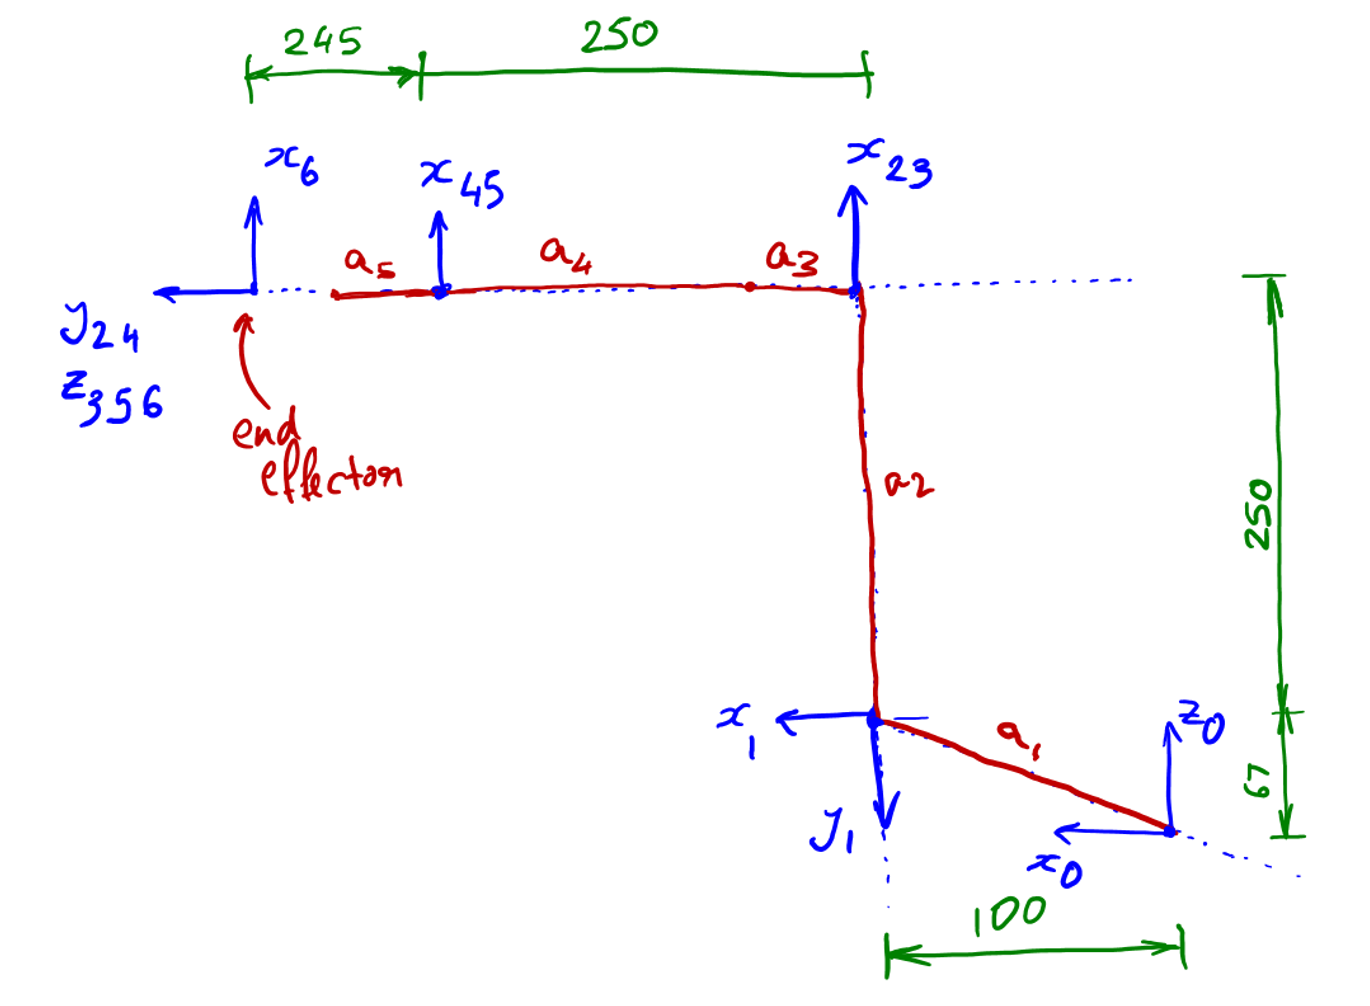
\includegraphics[scale=0.5]{q3}\\
				\caption [DHDrawing]{D-H Standard for Forward Kinematics Coordinate Systems}
			\end{centering}
		\end{figure}
		
	\pagebreak	
	\subsection*{Resulting Transformation Matrix}
	The resulting transformation matrix can be represented as:\\
		\begin{center}
			\bf{^{0}T_{6}} =
			\begin{pmatrix}
				n_{x} & s_{x} & a_{x} & p_{x}\\
				n_{y} & s_{y} & a_{y} & p_{y}\\
				n_{z} & s_{z} & a_{z} & p_{z}\\
				0	&	0	&	0	&	1
			\end{pmatrix}
			$ = {^{0}A_{1}}\mult{^{1}A_{2}}\mult{^{2}A_{3}}\mult{^{3}A_{4}}\mult{^{4}A_{5}}\mult{^{5}A_{6}}$
		\end{center}
		\vspace{5mm}
	\flushleft
\bf{n_{x}} =
$$
- \sin\theta_{6}\mult (\cos\theta_{4}\mult \sin\theta_{1} - \sin\theta_{4}\mult (\cos\theta_{1}\mult \sin\theta_{2}\mult \sin\theta_{3} - \cos\theta_{1}\mult \cos\theta_{2}\mult \cos\theta_{3}))-  \cos\theta_{6}\mult (\cos\theta_{5}\mult (\sin\theta_{1}\mult \sin\theta_{4} + \cos\theta_{4}\mult (\cos\theta_{1}\mult \sin\theta_{2}\mult \sin\theta_{3} - \cos\theta_{1}\mult \cos\theta_{2}\mult \cos\theta_{3})) + \sin\theta_{5}\mult (\cos\theta_{1}\mult \cos\theta_{2}\mult \sin\theta_{3} + \cos\theta_{1}\mult \cos\theta_{3}\mult \sin\theta_{2}))
$$\vspace{3mm}

\bf{s_{x}} = 
$$
\sin\theta_{6}\mult (\cos\theta_{5}\mult (\sin\theta_{1}\mult \sin\theta_{4} + \cos\theta_{4}\mult (\cos\theta_{1}\mult \sin\theta_{2}\mult \sin\theta_{3} - \cos\theta_{1}\mult \cos\theta_{2}\mult \cos\theta_{3})) + \sin\theta_{5}\mult (\cos\theta_{1}\mult \cos\theta_{2}\mult \sin\theta_{3} + \cos\theta_{1}\mult \cos\theta_{3}\mult \sin\theta_{2})) - \cos\theta_{6}\mult (\cos\theta_{4}\mult \sin\theta_{1} - \sin\theta_{4}\mult (\cos\theta_{1}\mult \sin\theta_{2}\mult \sin\theta_{3} - \cos\theta_{1}\mult \cos\theta_{2}\mult \cos\theta_{3}))
$$\vspace{3mm}


\bf{a_{x}} =
$$
\sin\theta_{5}\mult (\sin\theta_{1}\mult \sin\theta_{4} + \cos\theta_{4}\mult (\cos\theta_{1}\mult \sin\theta_{2}\mult \sin\theta_{3} - \cos\theta_{1}\mult \cos\theta_{2}\mult \cos\theta_{3})) - \cos\theta_{5}\mult (\cos\theta_{1}\mult \cos\theta_{2}\mult \sin\theta_{3} + \cos\theta_{1}\mult \cos\theta_{3}\mult \sin\theta_{2})
$$\vspace{3mm}

\bf{p_{x}} = 
$$
100\mult \cos\theta_{1} + 250\mult \cos\theta_{1}\mult \cos\theta_{2} - 250\mult \sin\theta_{1}\mult \sin\theta_{4} - 250\mult \sin\theta_{6}\mult (\cos\theta_{4}\mult \sin\theta_{1} - \sin\theta_{4}\mult (\cos\theta_{1}\mult \sin\theta_{2}\mult \sin\theta_{3} - \cos\theta_{1}\mult \cos\theta_{2}\mult \cos\theta_{3})) - 250\mult \cos\theta_{6}\mult (\cos\theta_{5}\mult (\sin\theta_{1}\mult \sin\theta_{4} + \cos\theta_{4}\mult (\cos\theta_{1}\mult \sin\theta_{2}\mult \sin\theta_{3} - \cos\theta_{1}\mult \cos\theta_{2}\mult \cos\theta_{3})) + \sin\theta_{5}\mult (\cos\theta_{1}\mult \cos\theta_{2}\mult \sin\theta_{3} + \cos\theta_{1}\mult \cos\theta_{3}\mult \sin\theta_{2})) - 250\mult \cos\theta_{4}\mult (\cos\theta_{1}\mult \sin\theta_{2}\mult \sin\theta_{3} - \cos\theta_{1}\mult \cos\theta_{2}\mult \cos\theta_{3})
$$\vspace{3mm}

\bf{n_{y}} =
$$
\sin\theta_{6}\mult (\cos\theta_{1}\mult \cos\theta_{4} + \sin\theta_{4}\mult (\sin\theta_{1}\mult \sin\theta_{2}\mult \sin\theta_{3} - \cos\theta_{2}\mult \cos\theta_{3}\mult \sin\theta_{1})) + \cos\theta_{6}\mult (\cos\theta_{5}\mult (\cos\theta_{1}\mult \sin\theta_{4} - \cos\theta_{4}\mult (\sin\theta_{1}\mult \sin\theta_{2}\mult \sin\theta_{3} - \cos\theta_{2}\mult \cos\theta_{3}\mult \sin\theta_{1})) - \sin\theta_{5}\mult (\cos\theta_{2}\mult \sin\theta_{1}\mult \sin\theta_{3} + \cos\theta_{3}\mult \sin\theta_{1}\mult \sin\theta_{2}))
$$\vspace{3mm}



\bf{s_{y}} =
$$
\cos\theta_{6}\mult (\cos\theta_{1}\mult \cos\theta_{4} + \sin\theta_{4}\mult (\sin\theta_{1}\mult \sin\theta_{2}\mult \sin\theta_{3} - \cos\theta_{2}\mult \cos\theta_{3}\mult \sin\theta_{1})) - \sin\theta_{6}\mult (\cos\theta_{5}\mult (\cos\theta_{1}\mult \sin\theta_{4} - \cos\theta_{4}\mult (\sin\theta_{1}\mult \sin\theta_{2}\mult \sin\theta_{3} - \cos\theta_{2}\mult \cos\theta_{3}\mult \sin\theta_{1})) - \sin\theta_{5}\mult (\cos\theta_{2}\mult \sin\theta_{1}\mult \sin\theta_{3} + \cos\theta_{3}\mult \sin\theta_{1}\mult \sin\theta_{2}))
$$\vspace{3mm}

\bf{a_{y}} = 
$$
- \sin\theta_{5}\mult (\cos\theta_{1}\mult \sin\theta_{4} - \cos\theta_{4}\mult (\sin\theta_{1}\mult \sin\theta_{2}\mult \sin\theta_{3} - \cos\theta_{2}\mult \cos\theta_{3}\mult \sin\theta_{1})) - \cos\theta_{5}\mult (\cos\theta_{2}\mult \sin\theta_{1}\mult \sin\theta_{3} + \cos\theta_{3}\mult \sin\theta_{1}\mult \sin\theta_{2})
$$\vspace{3mm}

\bf{p_{y}} =
$$
100\mult \sin\theta_{1} + 250\mult \cos\theta_{2}\mult \sin\theta_{1} + 250\mult \cos\theta_{1}\mult \sin\theta_{4} + 250\mult \sin\theta_{6}\mult (\cos\theta_{1}\mult \cos\theta_{4} + \sin\theta_{4}\mult (\sin\theta_{1}\mult \sin\theta_{2}\mult \sin\theta_{3} - \cos\theta_{2}\mult \cos\theta_{3}\mult \sin\theta_{1})) - 250\mult \cos\theta_{4}\mult (\sin\theta_{1}\mult \sin\theta_{2}\mult \sin\theta_{3} - \cos\theta_{2}\mult \cos\theta_{3}\mult \sin\theta_{1}) + 250\mult \cos\theta_{6}\mult (\cos\theta_{5}\mult (\cos\theta_{1}\mult \sin\theta_{4} - \cos\theta_{4}\mult (\sin\theta_{1}\mult \sin\theta_{2}\mult \sin\theta_{3} - \cos\theta_{2}\mult \cos\theta_{3}\mult \sin\theta_{1})) - \sin\theta_{5}\mult (\cos\theta_{2}\mult \sin\theta_{1}\mult \sin\theta_{3} + \cos\theta_{3}\mult \sin\theta_{1}\mult \sin\theta_{2}))
$$\vspace{3mm}

\bf{n_{z}} = 
$$
\cos\theta_{6}\mult (\sin\theta_{5}\mult (\cos\theta_{2}\mult \cos\theta_{3} - \sin\theta_{2}\mult \sin\theta_{3}) + \cos\theta_{4}\mult \cos\theta_{5}\mult (\cos\theta_{2}\mult \sin\theta_{3} + \cos\theta_{3}\mult \sin\theta_{2})) - \sin\theta_{4}\mult \sin\theta_{6}\mult (\cos\theta_{2}\mult \sin\theta_{3} + \cos\theta_{3}\mult \sin\theta_{2})
$$\vspace{3mm}

\bf{s_{z}} = 
$$
- \sin\theta_{6}\mult (\sin\theta_{5}\mult (\cos\theta_{2}\mult \cos\theta_{3} - \sin\theta_{2}\mult \sin\theta_{3}) + \cos\theta_{4}\mult \cos\theta_{5}\mult (\cos\theta_{2}\mult \sin\theta_{3} + \cos\theta_{3}\mult \sin\theta_{2})) - \cos\theta_{6}\mult \sin\theta_{4}\mult (\cos\theta_{2}\mult \sin\theta_{3} + \cos\theta_{3}\mult \sin\theta_{2})
$$\vspace{3mm}

\bf{a_{z}} = 
$$
\cos\theta_{5}\mult (\cos\theta_{2}\mult \cos\theta_{3} - \sin\theta_{2}\mult \sin\theta_{3}) - \cos\theta_{4}\mult \sin\theta_{5}\mult (\cos\theta_{2}\mult \sin\theta_{3} + \cos\theta_{3}\mult \sin\theta_{2})
$$\vspace{3mm}

\bf{p_{z}} = 
$$
250\mult \sin\theta_{2} + 250\mult \cos\theta_{6}\mult (\sin\theta_{5}\mult (\cos\theta_{2}\mult \cos\theta_{3} - \sin\theta_{2}\mult \sin\theta_{3}) + \cos\theta_{4}\mult \cos\theta_{5}\mult (\cos\theta_{2}\mult \sin\theta_{3} + \cos\theta_{3}\mult \sin\theta_{2})) + 250\mult \cos\theta_{4}\mult (\cos\theta_{2}\mult \sin\theta_{3} + \cos\theta_{3}\mult \sin\theta_{2}) - 250\mult \sin\theta_{4}\mult \sin\theta_{6}\mult (\cos\theta_{2}\mult \sin\theta_{3} + \cos\theta_{3}\mult \sin\theta_{2}) + 67
$$\vspace{3mm}
	